\section{Results}\label{sec:pre}
The real parameters are $a=(0.1, -0.2, 0.2)^T$, with initial conditions $z_0=(0,0,0,-0.1, -0.4,  0)^T$. In \cref{tab:params}, we present three different set of simulation parameters that were used, and the results are presented in \cref{fig:orig,fig:estimation,fig:estimation2}.


\begin{table}[H]
\centering
\begin{tabular}{llll}
\hline
\textbf{Set} & \textbf{\boldmath$C$} & \textbf{\boldmath$Q_t$} & \textbf{\boldmath$R_t$} \\ \hline
1            & $C_1$                 & $0.01 I_6$        & 25                      \\
2            & $C_2$                 & $I_6$                   & 5                       \\
3            & $C_3$                 & $I_6$                   & $5 I_3$           \\ \hline
\end{tabular}
\caption{Parameters for estimation procedure.}
\label{tab:params}
\end{table}
where
\[
\begin{split}
C_1&=\begin{bmatrix}
  1 & 0 & 0 & 0 & 0 & 0
\end{bmatrix}\\
C_2&=\begin{bmatrix}
  1 & 1 & 1 & 0 & 0 & 0
\end{bmatrix}\\
C_3&=\begin{bmatrix}
  1 & 0 & 0 & 0 & 0 & 0\\
  0 & 1 & 0 & 0 & 0 & 0\\
  0 & 0 & 1 & 0 & 0 & 0\\
\end{bmatrix}.
\end{split}
\]

\begin{figure}[H]
  \centering
  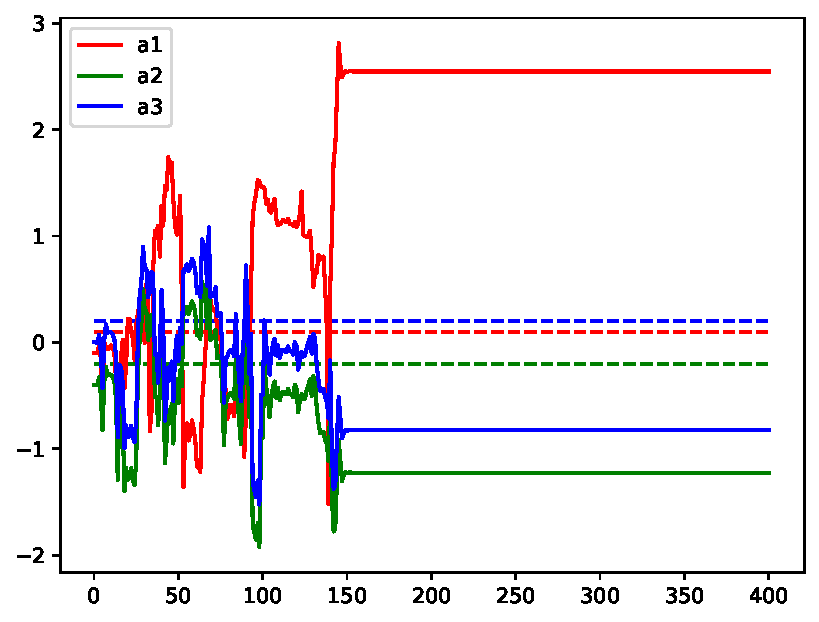
\includegraphics[scale=.4]{files/chinese_original.pdf}
  \caption{Parameter estimation using EKF for set 1.}
  \label{fig:orig}
\end{figure}

\begin{figure}[H]
  \centering
  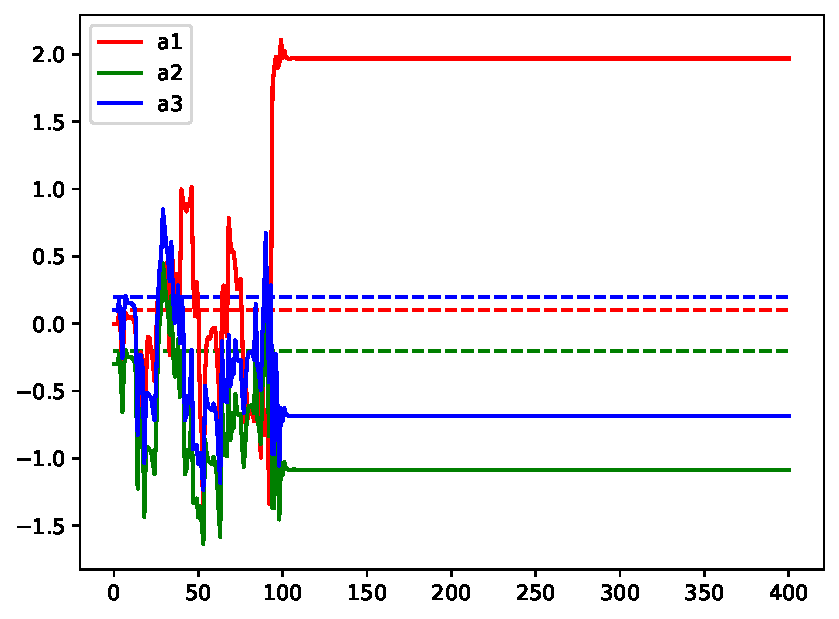
\includegraphics[scale=.4]{files/chinese_estimation.pdf}
  \caption{Parameter estimation using EKF for set 2.}
  \label{fig:estimation}
\end{figure}

\begin{figure}
  \centering
  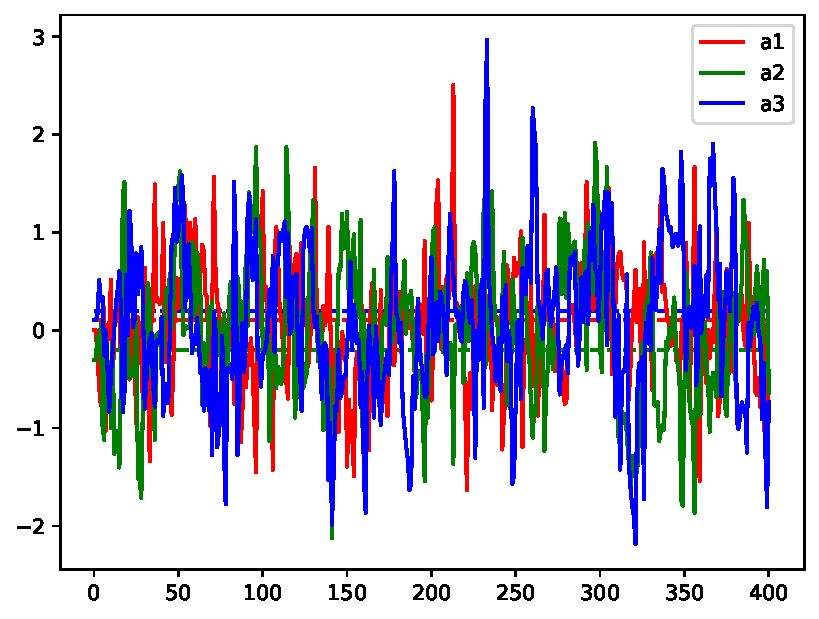
\includegraphics[scale=.4]{files/chinese_estimation_2.pdf}
  \caption{Parameter estimation using EKF for set 3.}
  \label{fig:estimation2}
\end{figure}

The results for set 1 (\cref{fig:orig}) show that the estimation does not present significant dynamics, therefore the parameters do not converge to the real values. This possible occurs since $Q_t$ is small; after testing with more scattered noises, we obtained more movement only in the parameter $a_1$, which is associated with the first equation that is also the output.


Attempting to solve this problem, we propose the set 2 and 3, on which the output includes all the original states. Consequently, more changes in the estimated parameters were obtained, but it did not converge to the desired value.
